% Uncomment the following line to have comments hihglighted
\documentclass[10pt]{extarticle}
% Uncomment the following line to disable comments and highlights
% \documentclass[9pt,final]{extarticle}

% To use colours
\usepackage[usenames,dvipsnames]{xcolor}
% To nicely format URLs
\usepackage{url}
\usepackage[pdftex]{graphicx}
\usepackage{epstopdf}
\setkeys{Gin}{draft=false}

% For using inparaenum, basically
\usepackage{paralist}
% For adding TODO notes
\usepackage[obeyDraft,textsize=tiny,backgroundcolor=blue!10]{todonotes}
% To 
% \usepackage[square,numbers,sectionbib]{natbib}
% To add author blocks to the front-matter
\usepackage{authblk}

%bibliography
\usepackage{natbib}

% To create linked anchors on top of references
%\usepackage[pdfborder={0 0 0}]{hyperref}
% To play around with enumerations and bullet lists
\usepackage{enumitem}
% To load hyphenation rules and other Locale-standardised things
\usepackage[british]{babel}
% For the letter-like symbol, {\Letter}
\usepackage{marvosym}
% To comment
\usepackage{comment}
% To adjust margins
\usepackage{geometry}
% Fancy HREFs
\usepackage[draft=true]{hyperref}
%\usepackage{nohyperref}
% Fancy enumerations and itemised lists
\usepackage{enumitem}
% For \mathbb command, among the others
\usepackage{amsfonts}
% For creating side-notes
\usepackage{marginnote}
% For specifying kewords and acronyms
\usepackage[nonumberlist,acronym,sanitize=none]{glossaries}
\glsdisablehyper
% For equations, arrays of equations, defining operator names, etc.
\usepackage{amsmath}
% For cursive math
\usepackage{mathrsfs}
% For math symbols, such as \nexists
\usepackage{amssymb}
% To check whether the document is in its final version or not
\usepackage{ifdraft}
% To highlight text
\usepackage{soul}
% For a decent formatting of numbers (and a wonderful system for numeric columns in tables, ``S'')
\usepackage{siunitx}
% To create right arrows in the text environment
\usepackage{textcomp}
% For smart references
\usepackage[capitalise,nameinlink]{cleveref}
% To cross-reference other documents
\usepackage{xr}

% requires packages:
% To check whether the document is in its final version or not
\RequirePackage{ifdraft}
% To color text
\RequirePackage{xcolor}
% To make smart references
\RequirePackage{cleveref}
%
\geometry{
 a4paper,
 total={210mm,297mm},
 left=15mm,
 right=15mm,
 top=15mm,
 bottom=25mm,
 marginparwidth=15mm
}
%
\renewcommand\Affilfont{\itshape\small}

% Counter for comments
\newcounter{commentcnt}
% Refine the comment counters by using the Roman numbering system. Notice that the new counter {commentcnt} automatically creates \thecommentcnt as a new command, which has to be overwritten.
\renewcommand{\thecommentcnt}{\arabic{commentcnt}}
% To use cleveref with this environment
\Crefname{commentcnt}{Comment}{Comment}

\newenvironment{ReviewerComment}[2][]{\noindent\begin{minipage}[t]{\textwidth}\noindent \textbf{Comment \refstepcounter{commentcnt}{\thecommentcnt} %
% If an optional argument is passed, it is used as the label of the environment
\ifx\empty#1\relax\else#1\fi%
(Reviewer #2): } \begin{quotation}\noindent}{\end{quotation}\vspace{1ex}\end{minipage}}
%
\newenvironment{ReviewerCommentReprise}{\noindent\vspace{-1.25cm}%
\begin{quotation}\noindent\begin{em}}{\end{em}\end{quotation}}
%
\newenvironment{ReviewerReply}{\noindent \textbf{Feedback: } \begin{quotation}\begin{em}}{\end{em}\end{quotation}}
%
\newenvironment{GuestEditorComment}{\noindent\begin{minipage}[t]{\textwidth}\noindent \textbf{Comment \refstepcounter{commentcnt}{\thecommentcnt} (Guest Editor): } \begin{quotation}\noindent\begin{em}}{\end{em}\end{quotation}\vspace{1ex}\end{minipage}}
%
\newenvironment{AreaEditorComment}{\noindent\begin{minipage}[t]{\textwidth}\noindent \textbf{Comment \refstepcounter{commentcnt}{\thecommentcnt} (Area Editor): }\nopagebreak \begin{quotation}\noindent\begin{em}}{\end{em}\end{quotation}\vspace{1ex}\end{minipage}}
%
\newenvironment{EditorComment}{\noindent\begin{minipage}[t]{\textwidth}\noindent \textbf{Comment \refstepcounter{commentcnt}{\thecommentcnt} (Editor in Chief): } \begin{quotation}\noindent\begin{em}}{\end{em}\end{quotation}\vspace{1ex}\end{minipage}}
%
\newenvironment{MetaReviewComment}{\noindent\begin{minipage}[t]{\textwidth}\noindent \textbf{Comment \refstepcounter{commentcnt}{\thecommentcnt} (Meta-review): } \begin{quotation}\noindent\begin{em}}{\end{em}\end{quotation}\vspace{1ex}\end{minipage}}
%
\newenvironment{Answer}{\noindent \textbf{Answer: }}{\\[1cm]}
%
\newenvironment{AnswerInBetween}{\noindent \textbf{Answer: }}{\vspace{1cm}}
%
% \newcommand{\NoteInEvidence}[1]{\color{GreenYellow}{\textbf{#1}}}


\newcommand{\NoteInEvidence}[1]{\ifoptiondraft{\hl{#1}}{}}


%bibliography directory
\newcommand\dirbiblio{../../../BIBLIO/}
%numbering of figures
%\renewcommand{\thefigure}{S\@arabic\c@figure}

%%%%%%%%%%%%%%%%%%%%%%%%%%%%%%%%%%%%%%%%%%%%%%%%%%%%%%%%%%%%%%%%
%
% Task difficulty assessment and work status boxes
%
%%%%%%%%%%%%%%%%%%%%%%%%%%%%%%%%%%%%%%%%%%%%%%%%%%%%%%%%%%%%%%%%
\newcommand{\TaskEstimationBox}[2]{%
\ifoptiondraft{\newline \parbox{1.0\linewidth}{\hfill \hfill {\colorbox{#2}{\color{White} \textbf{#1}}}}}%
{}%
}
%
\def\WorkInProgressRevTask {\TaskEstimationBox{Work in progress}{Cyan}}
\def\AlmostDoneRevTask {\TaskEstimationBox{Almost there}{NavyBlue}}
\def\RevTaskDone {\TaskEstimationBox{Done}{Blue}}
%
\def\NotEstimatedRevTask {\TaskEstimationBox{Effort not estimated}{Gray}}
\def\EasyRevTask {\TaskEstimationBox{Feasible}{ForestGreen}}
\def\MediumRevTask {\TaskEstimationBox{Medium effort}{Orange}}
\def\TimeConsumingRevTask {\TaskEstimationBox{Time-consuming}{Bittersweet}}
\def\HardRevTask {\TaskEstimationBox{Hard one}{Sepia}}
\def\DeathRevTask {\TaskEstimationBox{Death}{Black}}
%
\newcommand{\Assignment}[1]{
%
\ifoptiondraft{%
\newline \parbox{1.0\linewidth}{\hfill \hfill \textbf{Personal commment:} #1}%
}{}%
}

%
%%%%%%%%%%%%%%%%%%%%%%%%%%%%%%%% Put some space to separate reviewers comments
%
\newcommand{\SkipSpaceForReviewerComments}{\vspace{1em}}

%
%%%%%%%%%%%%%%%%%%%%%%%%%%%%%%%% Add notes to be removed when the letter is not a draft any more
%
% To color text
\RequirePackage{xcolor}
\newenvironment{NoteForAuthors}%
  {\ifoptiondraft{%
      \noindent%
      \colorbox{gray}%
      {\color{white} Note: }%
      \color{orange}%
      \begin{em}%
    }{}%
  }%
  {\ifoptiondraft{%
      \normalcolor%
      \end{em}%
    }{}%
  }

%
%%%%%%%%%%%%%%%%%%%%%%%%%%%%%%%% Highlight changes in revised manuscripts
%
% To color text
\RequirePackage{xcolor}
% To create side-notes
\RequirePackage{marginnote}
% Change the following line for larger (or narrower) side spaces
\setlength{\marginparwidth}{1cm}
% Change the following line for bigger (or smaller) fonts
\renewcommand*{\marginfont}{\footnotesize}

\newenvironment{HlRev}[1][]{%
	% No hyperrefs here
	\begin{NoHyper}
		% Change the colour to olive green
		\color{OliveGreen}%
		% If an argument is passed, it is used as the number of the comment in a side note
		\ifx\newenvironment#1\newenvironment\else\marginnote{Comment #1}\fi%
		%
	}{%
		% Restores the normal colour
		\normalcolor%
		% Restores the normal hyperref behaviour
	\end{NoHyper}%
}
%
%%%%%%%%%%%%%%%%%%%%%%%%%%%%%%%%%%%%%%%%%%%%%%%%%%%%%%%%%%%%%%%%%%%%%%%%%
%



\usepackage{natbib}
% Defines the path for the main output file (so as to cross-reference sections, figures, table there, by prepending "paper:" to the original label )
\externaldocument[paper:]{../LNCS-skeleton/main}

\def\PaperTitle{The imbricated foreshock and aftershock activities of the Balsorano (Italy) M$_w$ 4.4 normal fault earthquake and implications for earthquake initiation}
\def\PaperId{{Response letter to review for manuscript D-20-00253}}
\def\Journal{{Seismological Research Letters}}

\def\AuthorsInLetter{H. S. S\'anchez\text{-}Reyes, D. Essing, E. Beauc\'e, and P. Poli}

\usepackage{hyperref}
%opening
\title{\textbf{\PaperTitle} \\ {\Large Revision notes}}
%
%
\author[1]{H. S. S\'anchez\text{-}Reyes %
  \thanks{Corresponding author \\
    {\Letter}~{ISTerre OSUG-C (Maison des Géosciences), 1381 rue de la Piscine, 38400 Saint Martin D'H\`eres, France} \\
    {\Email}~\texttt{\href{mailto:hugo.sanchez-reyes@univ-grenoble-alpes.fr}{hugo.sanchez-reyes@univ-grenoble-alpes.fr}} \\
    {\Telefon}~\textsf{+33 66 80 73 04}%
  }
}
%
\author[1]{D. Essing}
%
\author[2]{E. Beauc\'e}
%
\author[1]{P. Poli}

\affil[1]{Institute of Earth Sciences, University Grenoble Alpes, Grenoble \emph{38100}, France}
\affil[2]{Department of Earth, Atmospheric, and Planetary Sciences, Massachusetts Institute of Technology, Cambridge, MA, United States}

\date{\today}
\begin{document}

\maketitle

%\input{intro}
Dear Editorial Board,
\\[2em]
We greatly appreciate your time and effort dedicated to revise our submitted manuscript. We have worked in order to address all the suggestions and comments pointed out by the reviewers and the associated editor. In the following pages we provide a detailed response to all the comments related to this revision. In addition, we attached a PDF file tracking all the changes that have been made in the main paper. We hope that the applied revisions are satisfactory to the reviewers and the editorial board.
\\[2em]
Kind regards,
\begin{flushright}
\AuthorsInLetter
\end{flushright}\vfill
%\input{manuscriptinfo}
\section*{Manuscript information}

\begin{description}
\item[Number:] \PaperId
\item[Title:] ``\PaperTitle''
\item[Authors:] \AuthorsInLetter
\item[Submitted to:] \Journal
\end{description}
\vfill
\pagebreak

%\input{revision-notes/reviewer1}

%\SkipSpaceForReviewerComments

%\input{revision-notes/reviewer2}

%\SkipSpaceForReviewerComments


\renewcommand\thefigure{\arabic{figure}} 

%%%%%%%%%%%%%%%%%%%%%%%%%%%%%%%%%%%%%%%%%%%%%%%%%%%%%%%%%%%%%%%%%%%%%%%%%%%%%%%%%%%%%%%%%%%%%%%%%%%%%%%%%%%%%%%%%%%%%%%%%%%%%%


\section*{Associate Editor Comment}

We have received two excellent reviews of this manuscript. In general, the reviewers agree that the manuscript provides valuable analysis and results that are appropriate for publication at SRL. Reviewer 2 raises some questions about the details of the analysis and makes some suggestions that could lead to improvements in their results, while Reviewer 1 asks important questions about the implications of the results, in particular about whether or not the pattern observed for this earthquake sequence is unique or common.

\section*{Reviewer \#1}


\subsection*{Summary}

This study investigates a seismicity sequence associated with a Mw 4.4 in central Italy. They use network-matched-filtering (which includes waveform cross correlation), clustering, and relocation to detect a large number of earthquakes and then classify them into clusters. They find that one cluster involved a large number of events prior to the mainshock. The study provides an example of how to investigate a seismicity sequence when there is sufficient station coverage near the epicenter. The main questions, to me, are whether the interpretations are reliable (do the dots illuminate a fault?) and whether they are significant (is this earthquake novel, in the global sense)? The authors have done a great job motivating the study and establishing the literature. From my comments below, I suggest that major revisions would be needed. The scientific approach appears to be sound, but the presentation of results could be improved and expanded in order to justify the significance. \\

{\bf Key points (from author):} \\
\begin{itemize}
 \item[1] The analysis of the 2019 Balsorano earthquake sequence reveals that imbricated complex processes occur before and after the main earthquake. 
 \item[2] Clear differences between foreshocks and aftershocks are highlighted by the distinct spatio-temporal patterns unraveled by our analysis.
 \item[3] These results demonstrate that simple earthquake preparation models are not suitable enough to correctly mimic the observed complex reality.
\end{itemize}



\begin{ReviewerComment}{1}
\noindent 
Given the detailed study of this M4 earthquake, and also the relevance of the fault planes inferred from the focal mechanism, it would be good to display a figure showing the waveform fits between data and synthetics. Such a figure might be available already from INGV. Or maybe the authors can generate such a figure using an alternative code.
\end{ReviewerComment}


\begin{Answer}
We agree with reviewer \#1 about the importance of adding this relevant figure. We have included a modified version of the figures provided by the INGV (\url{http://webservices.ingv.it/webservices/ingv_ws_map/data/tdmt/15111/73711301_86_tdmt_reviewer_solution.pdf}) showing the estimated focal mechanism together with a comparison between observed and estimated synthetic sesimograms as part of the supplementary material (as figure S2). We also present here below this figure. The former figure S2 (from the previous version) was removed according to the following comments from reviewer \#2 and this new figure related to the focal mechanism and synthetic seismograms took its place.
\begin{figure}[!h]
\begin{center}
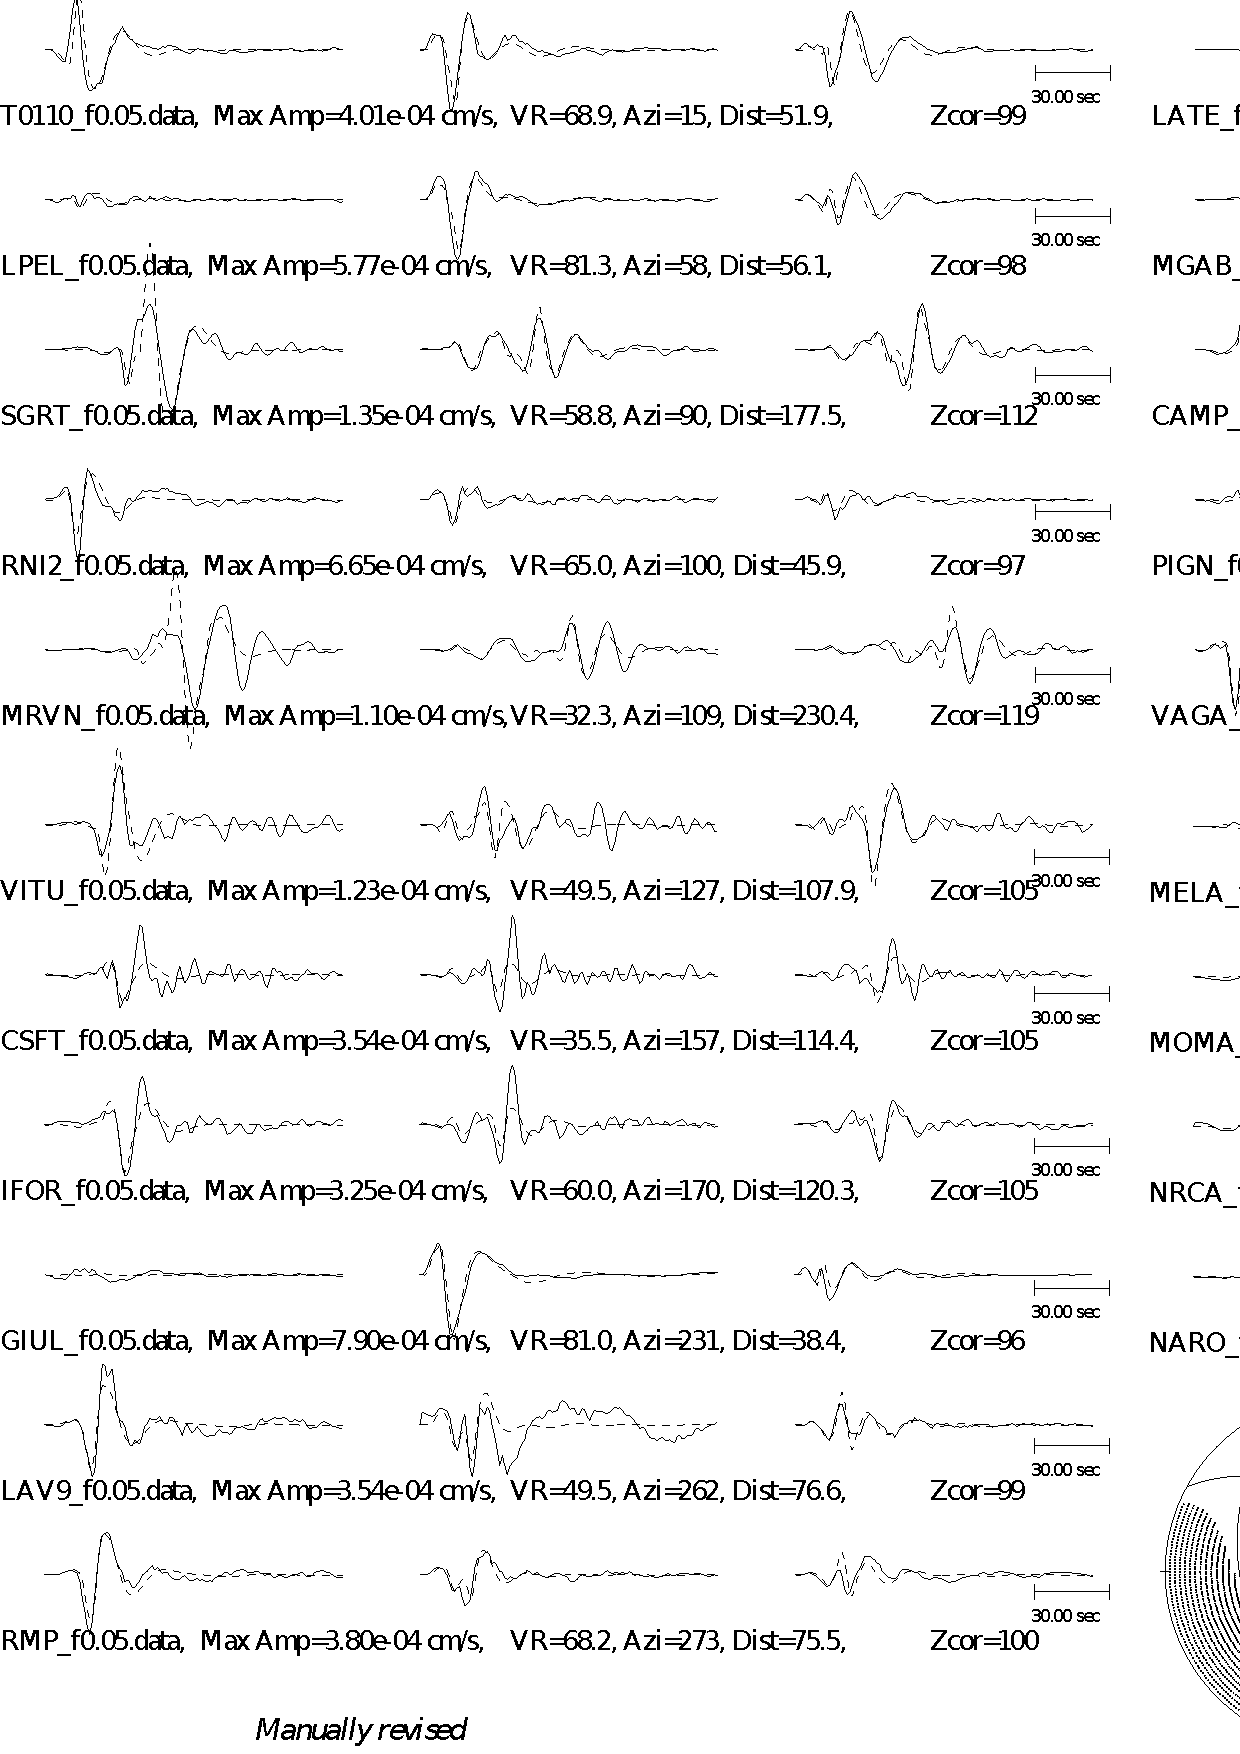
\includegraphics[width=1\linewidth]{S2_Focal_synthetics} 
\end{center}
\caption{Estimated focal mechanism and comparison of observed (solid lines) and estimated synthetic seismograms (dashed lines) for the Mw 4.4 mainshock. The three components at 22 receiver locations are shown. This figure is a modified version from the original one provided by the INGV \url{http://webservices.ingv.it/webservices/ingv_ws_map/data/tdmt/15111/73711301_86_tdmt_reviewer_solution.pdf}.}
\label{fig:S2_focal_mechanism}
\end{figure}
\Assignment{Hugo} \WorkInProgressRevTask
\end{Answer}
%
%



\begin{ReviewerComment}{1}
\noindent 
L104. "According to a geological study of the location of the main event and its focal mechanism (Supplementary Material Table S1), this event ruptured the Liri fault (Roberts and Michetti, 2004), which is one of the major active normal faults mapped in this region." \\

I did not see the evidence for choosing one of the two fault implied from the focal mechanism. (I looked in the supplement.) This is a critical piece, since the assumed fault plane is referenced in Figure 5.
\end{ReviewerComment}


\begin{Answer}
Thnaks for your comment. We consider that the evidence can be observed looking at the surface geololy. According to the work from \cite{Falcucci2016active}, which details the seismic active faults in this region, the second nodal plane from table S1 (strike 166$^o$, dip 42$^o$ and rake -51$^o$) coincides much better with the segment of the surface scarp of the normal Liri Fault. In order to emphasize the superficial scarp of the related Liri Fault, in the revised version we improve the former figure 1, increasing the resolution of the topography and including the observed fault scarp of the Liri fault reported by \cite{wedmore2017667}. We hope that this evidence is clearer in this version of the manuscript. This new figure is also included here below (as figure 2).
\begin{figure}[!h]
    \centering
     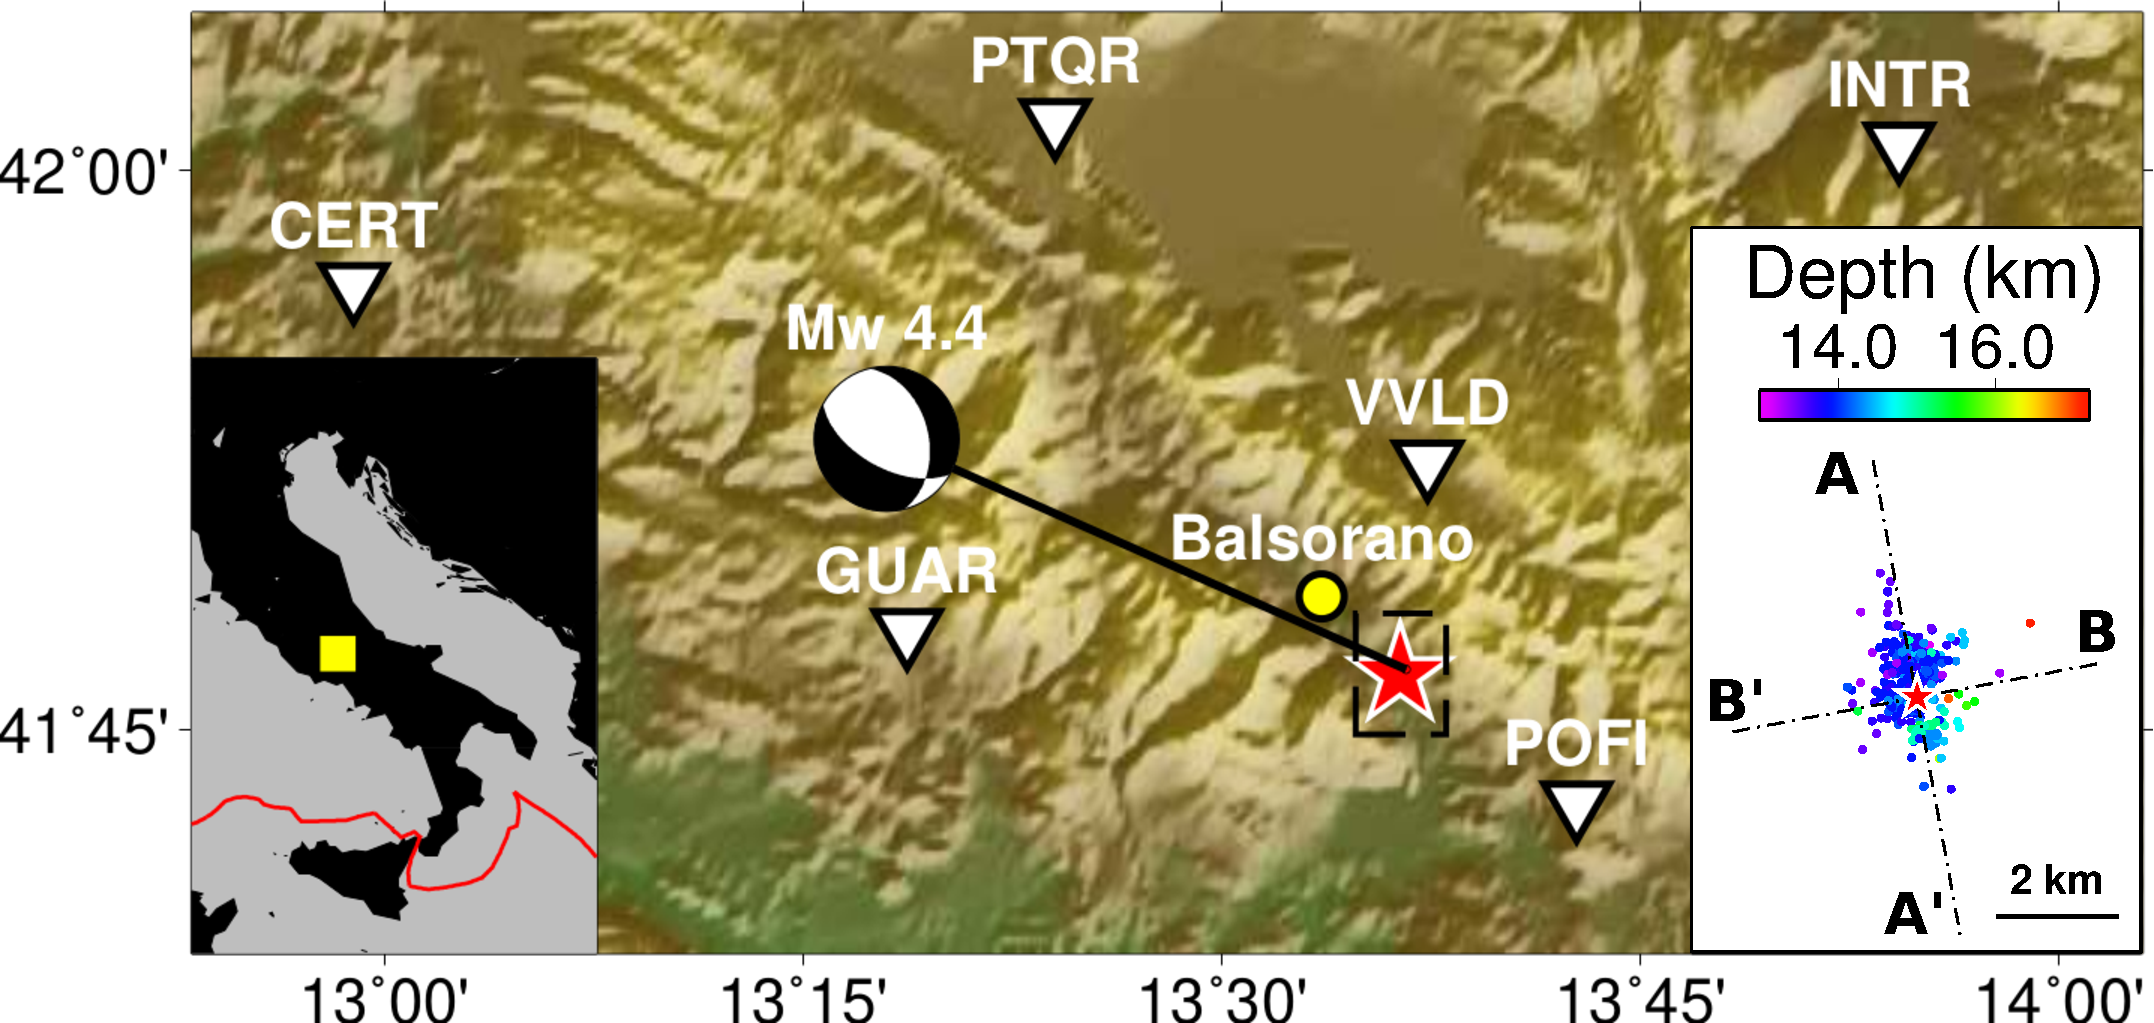
\includegraphics[width=1\linewidth]{map_balsorano.pdf}
    \caption{Regional map of the study area. The yellow square inside the small map inset on the left corresponds to the central region of Italy represented in the larger topographic map. The small map inset on the right represents magnification of the black dashed area around the epicentral location (red star). The color code used in the map view on the right represents the estimated depth of the foreshock and aftershock activity (estimated in this study: 714 events). The yellow circle represents Balsorano city, and the white triangles represent the stations used in this study. The dashed lines in the right inset map represent the directions A-A' (along strike) and B-B' (normal to the strike) illustrated in the cross sections of Figure 5. The solid red line represents the superficial scarp of the Liri fault (scarp taken from \cite{wedmore2017667}).}
\end{figure}
\Assignment{Hugo} \WorkInProgressRevTask
\end{Answer}
%
%



\begin{ReviewerComment}{1}
\noindent 
From one event, it is difficult to understand the significance of the findings. Did the authors point their same set of tools at a couple other events? What if all mainshocks in this region have foreshock sequences? What is the meaning of "normal" seismicity sequences in this region? In other words, is this one earthquake significant, or do many other earthquakes -- when examined this closely -- show such complexity? In particular, are there foreshock sequences such as Cluster 1?

\end{ReviewerComment}


\begin{Answer}
\hfill {\bf PIERO SAID HE WILL ANSWER THIS}
\Assignment{Hugo} \WorkInProgressRevTask
\end{Answer}
%
%



\begin{ReviewerComment}{1}
\noindent 
I have never done Coulomb stress modeling, but it seems like it was developed for this kind of study, where the fault is (likely) known, and the mechanism would predict aftershock occurrences in certain regions.
\end{ReviewerComment}


\begin{Answer}
We totally agree with reviewer \#1 about the potential of performing a Coulomb stress analysis in the region. However, the geometry of the faults, and subfaults, that were activated during this sequence are not known (except from the one associated to the mainshock). In addition, the focal mechanisms of most of the earthquakes in the sequence can not be determined due to their small size, noise levels and limitted azimuthal coverage. Finally, the slip distribution of the mainshock was not studied or inverted before. Therefore, the available information does not allow to perform a proper Coulomb stress analysis of this sequence. The above information is usually required by the available softwares performing such analysis \citep{toda2011coulomb}. We add (from lines 316 to 322) to the revised version a small paragaph listing the obstacles to perform such analysis for this sequence.
\Assignment{Hugo} \WorkInProgressRevTask
\end{Answer}
%
%



\begin{ReviewerComment}{1}
\noindent 
Figure 5 is key and needs improvements. There's too much white space to see the details.  Perhaps zoom into +/- 1 km and then leave the full +/- 3 km version in the supplement? No legend is needed, since the caption will tell us that a=Cluster1, b=Cluster2, etc. Save space by not displaying a, b, three times.
\end{ReviewerComment}


\begin{Answer}
We agree with reviewer \#1. We changed figure 5 in the revised version of the manuscript taking into account your comments and suggestions. We also include more information in this new version, such as the geometry of the auxiliary plane (NP1 in Table S1) and the location of the different templates belonging to each of the inferred clusters. You can also find the new version of this figure here below as figure 3.
\begin{figure}[!h]
\begin{center}
 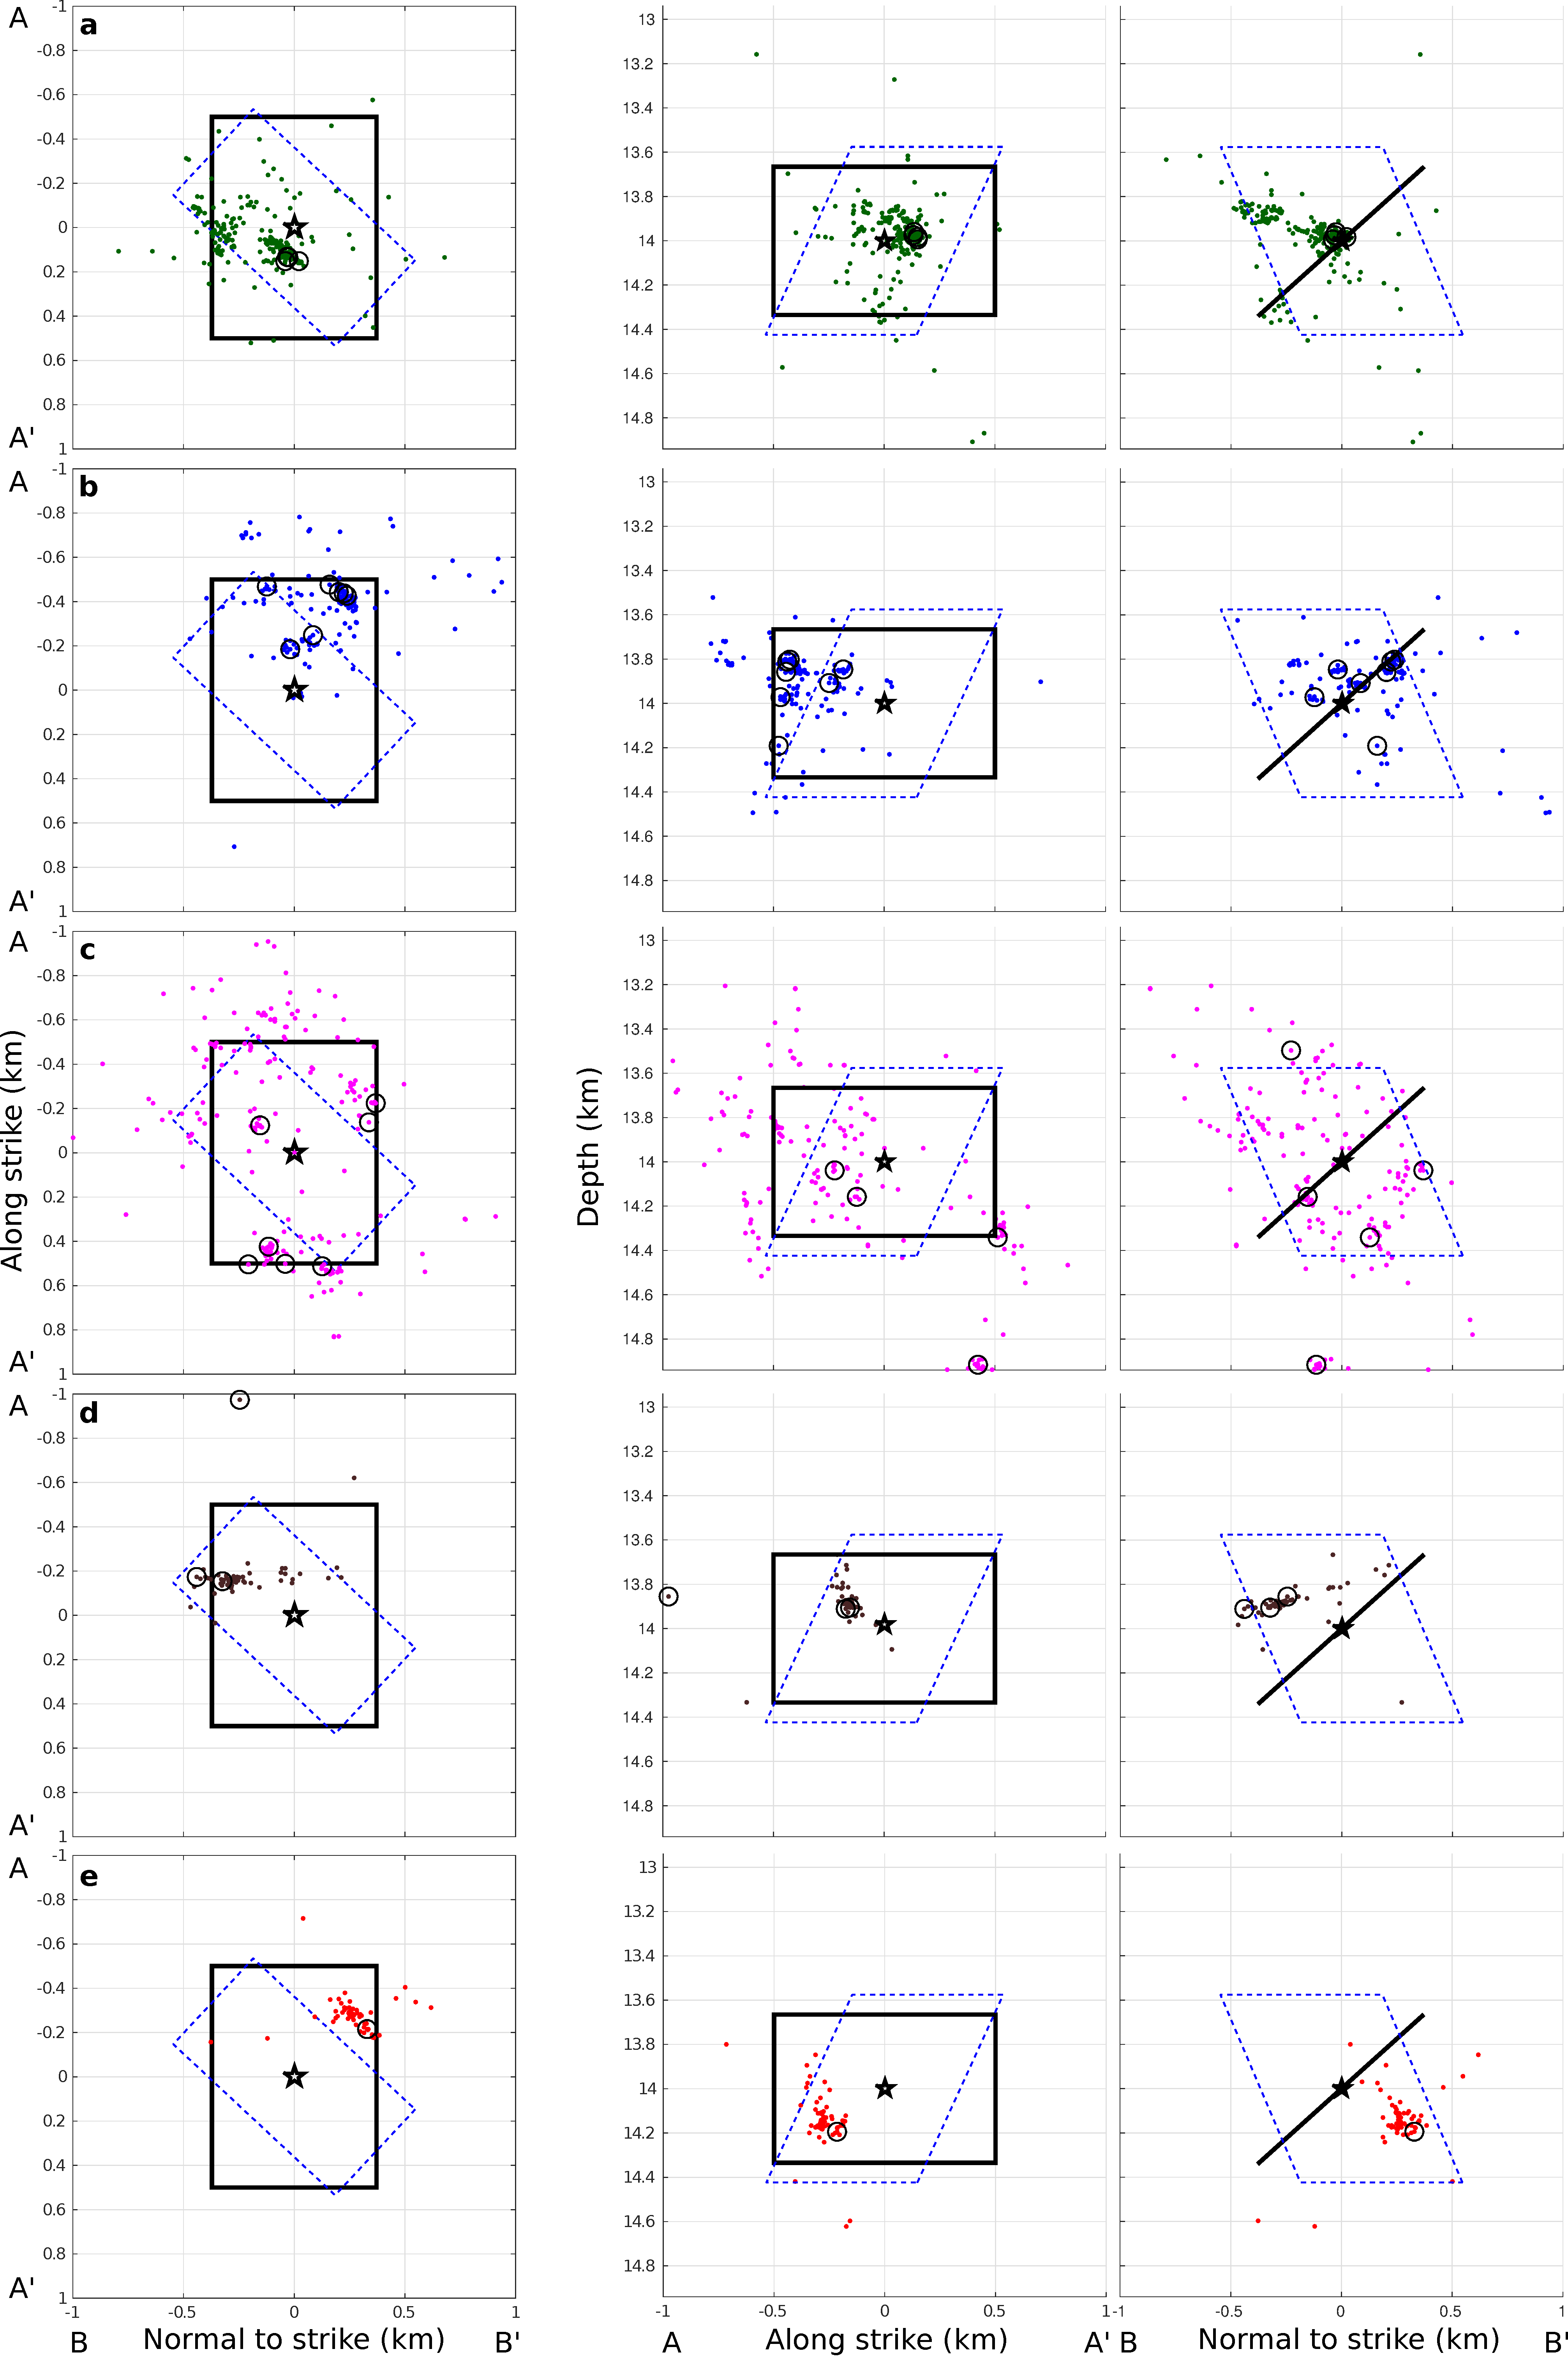
\includegraphics[width=0.75\linewidth]{map_clusters_templates}
\end{center}
\caption{Map view (left column), and cross-sections along the strike (middle column) and normal-strike (right column) directions for each of the five clusters identified in the sequence (as indicated). All of the locations are relative to the mainshock hypocenter (41.7746$^o$N 13.6066$^o$E; 13.94 km depth, black star). In all of the panels, the same color code is used as in Figures 3 and 4 to represent each different cluster. The solid black line represents a fault plane of 1 km$^2$ with the geometry of the second nodal plane (Supplementary Materials Table S1). The dashed blue line represents the assumed auxilary nodal plane. The directions A-A' (along strike) and B-B' (normal to the strike) are the same as in Figure 1. Each cluster is represented by a correponding label a) Cluster 1 , b) Cluster 2, c) Cluster 3, d) Cluster 4 and e) Cluster 5. In each panel, the black circles represent the location of the templates belonging to each cluster.}
\label{fig:map_improved}
\end{figure}
\Assignment{Hugo} \WorkInProgressRevTask
\end{Answer}
%
%


\begin{ReviewerComment}{1}
\noindent 
Figure 5a. Perhaps a dashed line for the assumed auxiliary plane? It is not clearcut to me that the dots are collapsing to a plane. (See also point about fault plane vs auxiliary plane above).
\end{ReviewerComment}


\begin{Answer}
We agree with reviewer \#1. We modified figure 5 in order to  illustrate both nodal planes as well as the relocated seismicity. This new figure is also included here as figure 3.
\Assignment{Hugo} \WorkInProgressRevTask
\end{Answer}
%
%


\begin{ReviewerComment}{1}
\noindent 
If the choice of fault plane is in question, then it would be good to see an alternative version of Figure 5, where the projection planes are chosen based on the now-assumed auxiliary plane (under the assumption that it is the mainshock fault plane).

\end{ReviewerComment}


\begin{Answer}
We think that the main fault plane is not under discussion thanks to the superficial evidence (from the new version of figure 1 in the main manuscript). However, we decide to show in figure 5 (main manuscript) also the auxiliary plane. You can find this new figure in this response letter as figure 3.
\Assignment{Hugo} \WorkInProgressRevTask
\end{Answer}
%
%


\begin{ReviewerComment}{1}
\noindent 
Most of the results imply complexity associated with the aftershock patterns. Is this exceptional? Are we to assume that the mainshock was complicated and that the aftershocks illuminate the region? Or that these adjacent faults were triggered by the mainshock?

\end{ReviewerComment}


\begin{Answer}
{\LARGE Not a good answer for this! I need help or some discussion!}
\Assignment{Hugo} \WorkInProgressRevTask
\end{Answer}
%
%




\begin{ReviewerComment}{1}
\noindent 
Fig. 2: mention diurnal variability in the white curve. Probably 6pm-6am or 18:00-06:00 is a better label. I don't think any legend is needed in b and c.

\end{ReviewerComment}


\begin{Answer}
Reviewer \#1 is right. We modified figure 2 in the new version of the main manuscript to take into account the given suggestions. This new version of the figure is part of this reponse letter as figure 4.
\Assignment{Hugo} \WorkInProgressRevTask
\begin{figure}[!h]
\begin{center}
 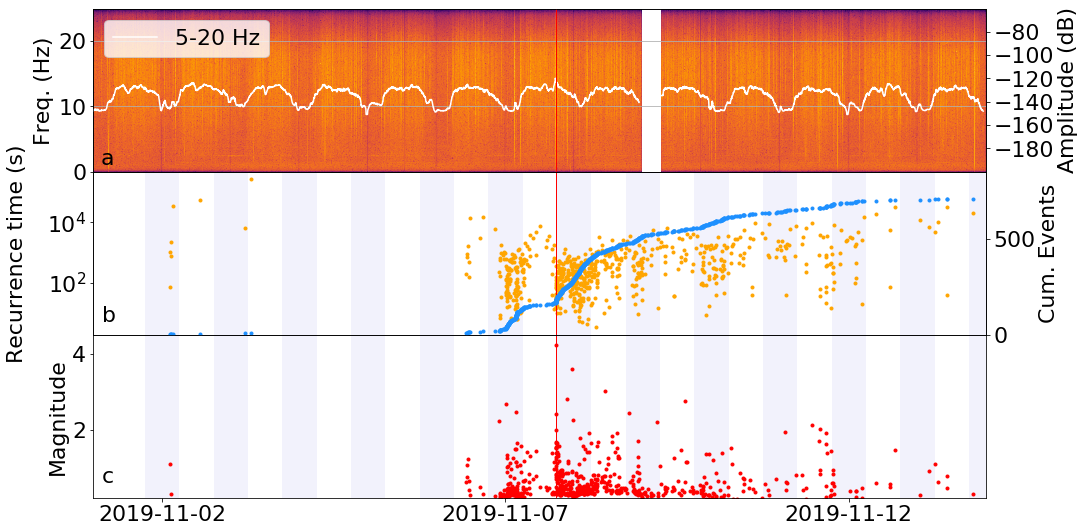
\includegraphics[width=1\linewidth]{spec_rec_mag.png} 
 \caption{(a) Spectrogram on VVLD.HHZ. The white line is the median of the energy in the frequency band between 5 Hz and 20 Hz calculated within a 1-h sliding window. Notice the diurnal energy variation. (b) Blue, cumulative events for the same time period of the experiment; orange, recurrence time for the newly detected events. (c) Estimated magnitudes for the newly detected events. A gap in the continuous data at this receiver location is seen for the night of November 8 to 9, 2019. In all pannels, day and night periods are represented by shaded (18:00 to 6:00) and unshaded (6:00 to 18:00) regions.}
\end{center}
\label{fig:new_fig_2}
\end{figure}
\end{Answer}
%
%


\begin{ReviewerComment}{1}
\noindent 
Figure 4. t=0 needs to be a tick mark, since that's the mainshock. (That way, you do not need the legend item for the mainshock either.)
\end{ReviewerComment}


\begin{Answer}
\Assignment{Hugo} \WorkInProgressRevTask
We agree with reviewer \#1. This suggestion is taken into account together with the following comment to modify figure 4 from the main manuscript (see figure 5 in this response letter).
\end{Answer}
%
%


\begin{ReviewerComment}{1}
\noindent 
Figure 4. I'm not finding the 90\% line to be helpful or representative of the distributions. Is it needed?
\end{ReviewerComment}


\begin{Answer}
\Assignment{Hugo} \WorkInProgressRevTask
We agree with reviewer \#1. This suggestion, and the previous one, are taken into account in the revised version of the main manuscript. This new figure is also included in this response letter as figure 5. We decide to leave the 90\% concentration line included in the right column of figure 4 (in main manuscript). We consider that this line illustrates the different ways that clusters behave and how their occurrence and location are particular to each group. In addition, the main manuscript makes reference to this line to stress out the different behaviors exhibited during the sequence.
\begin{figure}[!h]
\begin{center}
     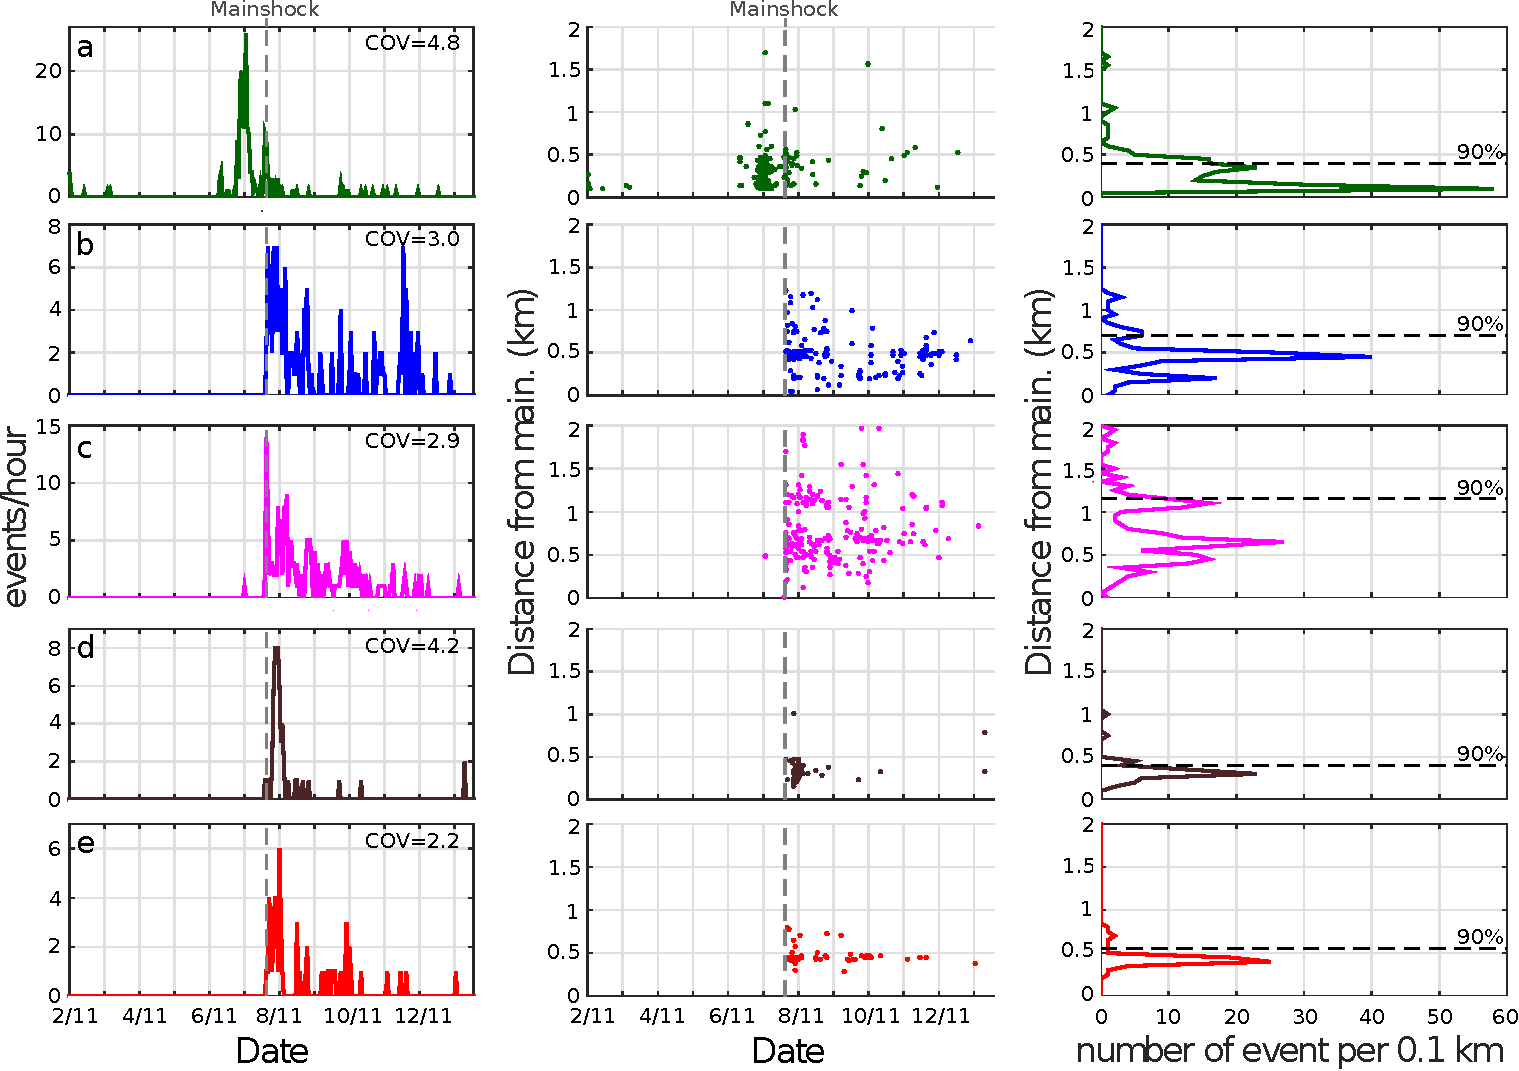
\includegraphics[width=1\linewidth]{densities_plot}         \caption{Spatio-temporal evolution of the earthquake sequences with respect to the mainshock origin time and hypocenter. Left column: Temporal density (number of events per hour). The coefficients of variation (COV) from the recurrence times are indicated for each cluster. Center column: Distance in time and space from each event of the sequence with respect to the mainshock location and origin time. The dashed grey line on the left and center column represents the mainshock origin time. Right column: Spatial density (concentration of events per 0.1 km). Dashed black line, where 90\% of the seismic activity is concentrated. (a)-(e) Each of the five clusters progresively ordered. The same color code from Figure 3 is used.}
\end{center}
\label{fig:new_fig_4}
\end{figure}
\end{Answer}
%
%

\section*{Reviewer \#2}

\subsection*{Summary}

This is an overall strong paper that is suitable for publication following minor edits. The authors perform a detailed analysis of foreshocks and aftershocks of the Mw 4.4 2019 Balsorano earthquake and demonstrate the complexity of these sequences, including apparent initiation on an antithetic fault. The authors first enhance the existing earthquake catalog using template matching. Next, they cluster events based on waveform similarity. Last, they relocate the majority of the newly detected events using the double-difference algorithm. The paper is clearly organized and the implications related to initiation processes and rupture complexities are very interesting.  \\


\subsection*{Template matching}

\begin{ReviewerComment}{2}
\noindent
Enhancing the catalog to 714 events is a significant improvement. However, using 23 out of 135 available catalog events as template earthquakes seems low and may prevent additional event detection. Is the 1-second pre-pick discussed on line 132 before the P-phase arrival? If so, why is the pre-pick time so long? This introduces noise to the signal - about 25% of the waveform - that decreases the signal-to-noise ratio that is then used in template selection. More templates would likely meet the SNR criteria with a shorter pre-pick, unless I misunderstand this 1-second pre-pick.

\end{ReviewerComment}


\begin{Answer}
We appreciate this comment. Regarding the 1-second pre-pick time window, we performed several tests with longer and shorter windows before defining the final duration of this window. Our results with longer windows totally agree with the comment from reviewer \#2, we had less detections and the correlation coefficients had lower values. In contrast, when shorter windows were used we did not see any significant increment of the number of detections. We did not exhaustively explore the results when shorter ($<$ 1 second) windows were used but the number of detections was not affected by this duration length.   
\Assignment{Hugo} \WorkInProgressRevTask
\end{Answer}
%
%

\begin{ReviewerComment}{1}
\noindent 
It would be helpful to provide the hypocentral locations and magnitudes of template events in Table S4, and include a map of template earthquakes to give a better idea whether detections (including the 13-15 km depth concentration of seismicity) are biased by template locations. Further, focal mechanisms of templates if available would provide additional information about potential biases in earthquake detection (i.e., if locations and focal mechanisms of templates are very similar, dissimilar events will not be detected). That being said, the results do not seem to be over-interpreted and a discussion of these potential biases would be adequate.

\end{ReviewerComment}


\begin{Answer}
We took into account these suggestions and we included more details of the 23 templates as part of the supplementary material (Table S5). In addition, we include also figure S6 to illustrate the relative location (with respect to the mainshock hypocenter) of the 23 templates. Furthermore, we modified figure 5 from the main manuscript to illustrate the location of the templates that belong to each of the different clusters composing the sequence. In this response letter, you can see these modification in figures.
\begin{figure}[!h]
\begin{center}
 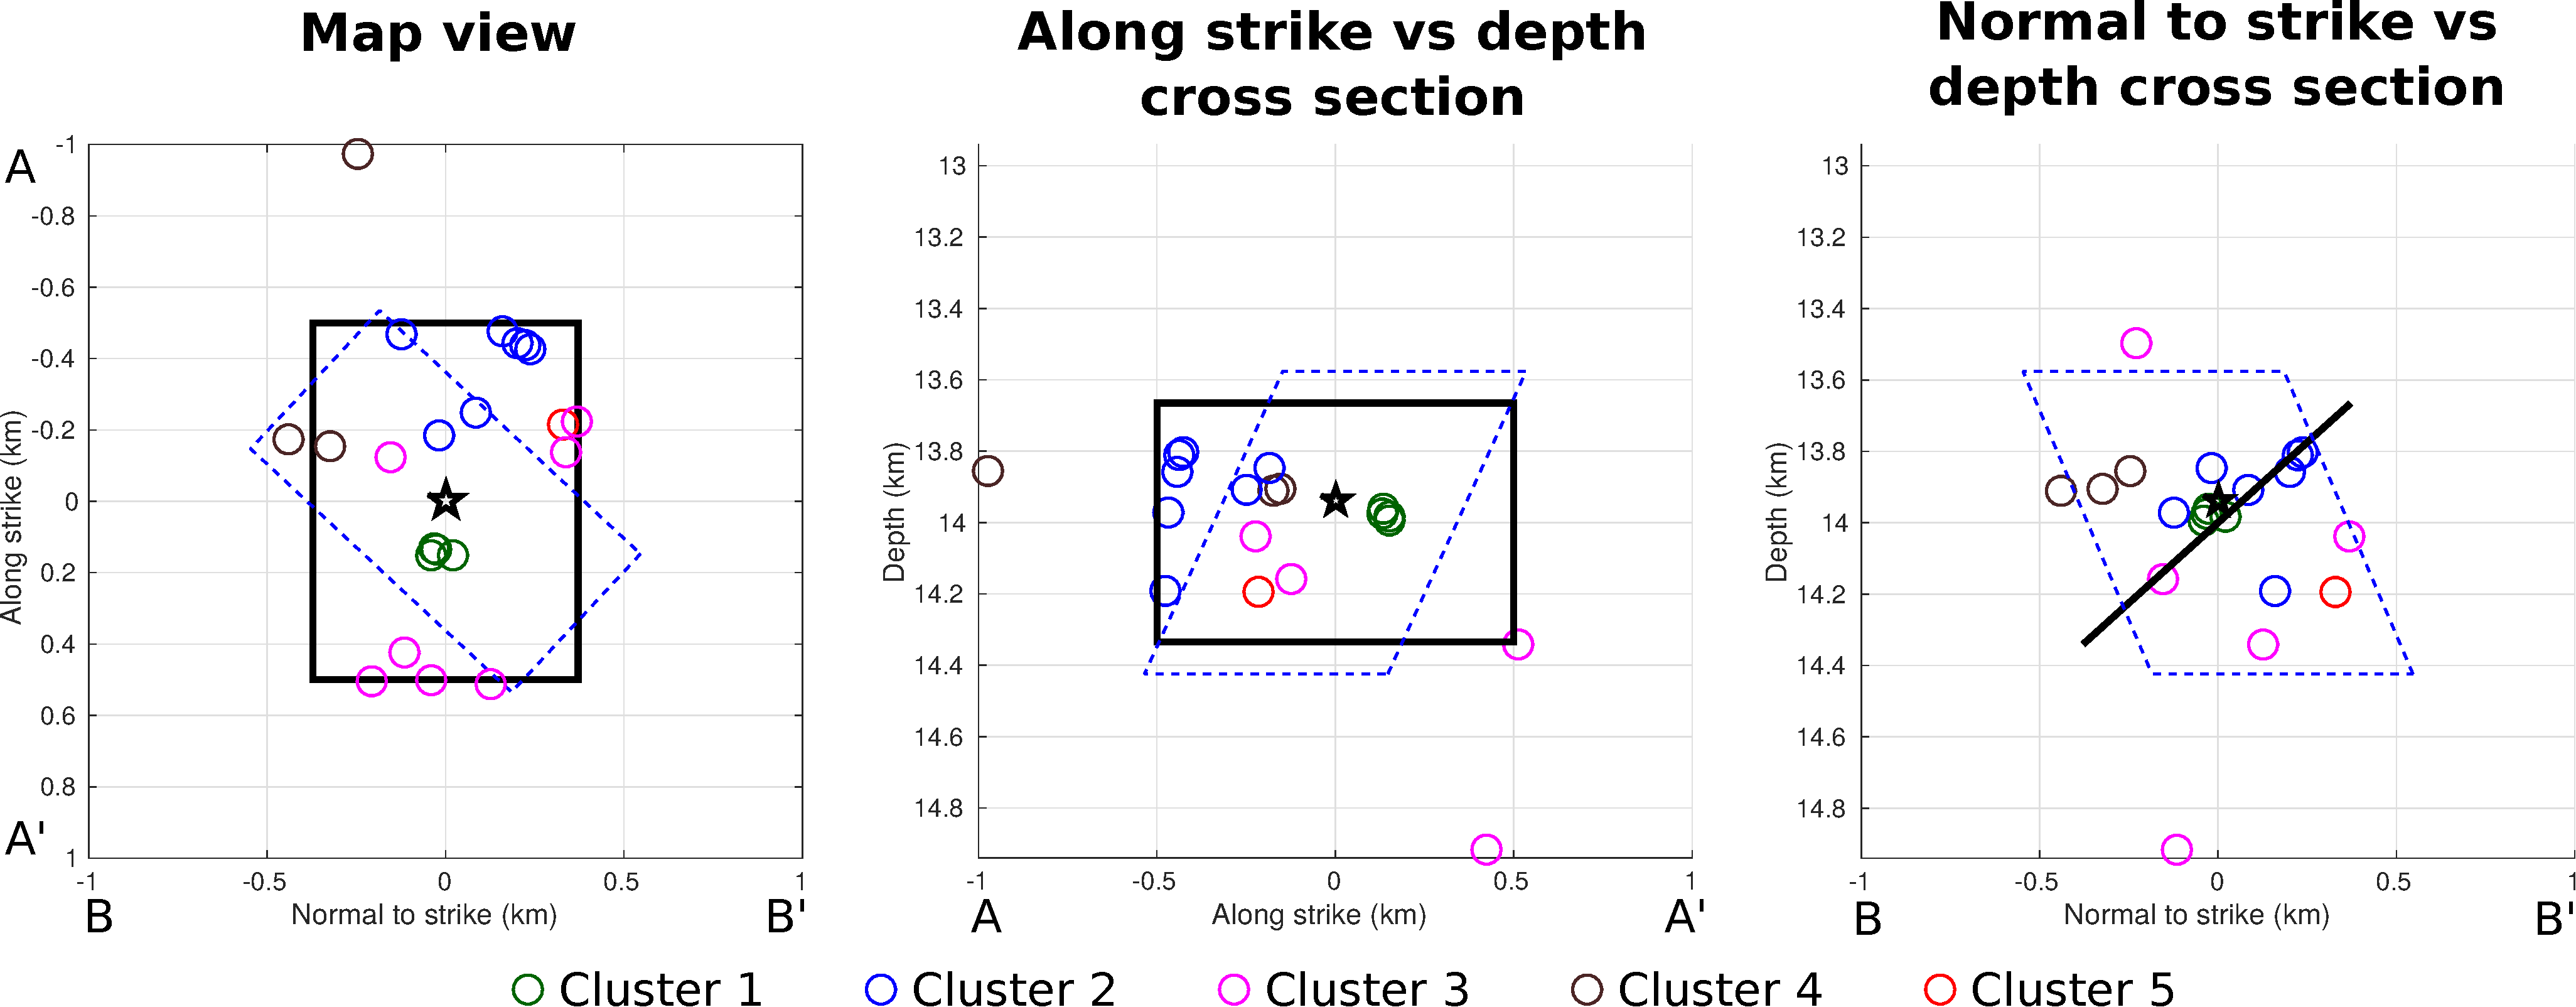
\includegraphics[width=1\linewidth]{S6_templates_per_cluster_map.pdf} 
\end{center}
\caption{Map view (left), and cross-sections along the strike (middle) and normal-strike (right) directions for the assumed main fault plane (solid black line). The dashed blue line illustrates the auxiliary plane listed in Table S1 (taken from the INGV moment tensor solution). The relative location of the 23 templates used for scanning the continuous recordings are represented by the center of the colored circles. The color code used defines to which cluster each of the templates belongs to. All of the locations are relative to the mainshock hypocenter (41.7746$^o$N 13.6066$^o$E; 13.94 km depth, black star). The directions A-A' (along strike) and B-B' (normal to the strike) are the same as in Figure 1 in the main manuscript.}
\label{fig:S6_templates_map}
\end{figure}
\Assignment{Hugo} \WorkInProgressRevTask
\end{Answer}
%
%



\begin{ReviewerComment}{2}
\noindent 
The method to determine the magnitude of earthquakes detected with template matching makes sense. However, the least-square fitting to obtain a linear model for magnitudes using only 23 earthquakes is unlikely to be robust. I suggest using more earthquakes in the INGV catalog to develop this model prior to applying it to the newly detected events.

\end{ReviewerComment}


\begin{Answer}
Thank you for this comment. We totally agree with reviewer \#2 about the possible lack of robustness of the newly estimated magnitudes. However, the estimated magnitudes are used only as a very cualitative measurement in our analysis. We do not use the estimated magnitudes to go further in our analysis or conclusions. Therefore, we think that the estimated magnitudes (using these 23 templates in the least squares model) are enogh accurate for the scope this study. We decided to include as part of the supplementary material figure S5, which illustrates the least squares model that we used for the magnitude estimation. This figure is also included in this response letter as figure \ref{fig:S5_lsq_model}.
\begin{figure}[!h]
\begin{center}
 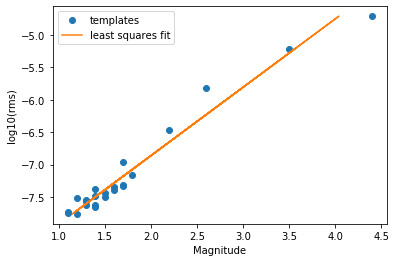
\includegraphics[width=0.7\linewidth]{S5_lsq_model.png} 
\end{center}
\label{fig:S5_lsq_model}
\end{figure}
\Assignment{Hugo} \WorkInProgressRevTask
\end{Answer}
%
%

\subsection*{Clustering}

\begin{ReviewerComment}{2}
\noindent 
Line 169 states that members of the same cluster should share similarities in position and rupture mechanism.  However, the locations in cluster 3 vary widely. The station nearest to the study region will not have large S-P time differences for most of the events; therefore, events in different locations with similar mechanisms might appear similar. Please expand on this in the waveform-based clustering section of methods, or consider using a farther station (or combining the results of multiple stations) for the waveform-based clustering.

\end{ReviewerComment}


\begin{Answer}
\Assignment{Hugo} \WorkInProgressRevTask
\end{Answer}
%
%



\begin{ReviewerComment}{2}
\noindent 
The stacked waveform for cluster 3 in Figure 3c is smaller amplitude than the other stacked waveforms and it is difficult to identify phase arrivals. This is likely because events in this cluster are not as similar as other clusters. Please discuss the similarity in this cluster more in the main text.

\end{ReviewerComment}


\begin{Answer}
\Assignment{Hugo} \WorkInProgressRevTask
\end{Answer}
%
%


\subsection*{Aseismic slip}


\begin{ReviewerComment}{2}
\noindent 
Pre-seismic: Line 302 in the Conclusion states that there is a lack of repeating earthquakes in the foreshock sequence. This should be mentioned earlier, perhaps near Lines 256-261 in the Results and Discussion section where the lack of evidence for aseismic slip is discussed.

\end{ReviewerComment}


\begin{Answer}
\Assignment{Hugo} \WorkInProgressRevTask
\end{Answer}
%
%



\begin{ReviewerComment}{2}
\noindent 
Post-seismic: Line 275 attributes clusters 4 and 5 to afterslip on the main fault. Afterslip can also trigger seismicity/aftershocks off of the main fault (Inbal et al., 2017) but this is still a reasonable mechanism. Is there a log(time) dependence in spatial expansion in these clusters that may also indicate aseismic slip? Are any repeating earthquakes present in the aftershock sequence that may be indicative of co-planar afterslip? I assume not since the foreshocks are the most highly correlated, but it is still worth mentioning in the discussion of afterslip as a mechanism.
\end{ReviewerComment}


\begin{Answer}
\begin{figure}[!h]
\begin{center}
 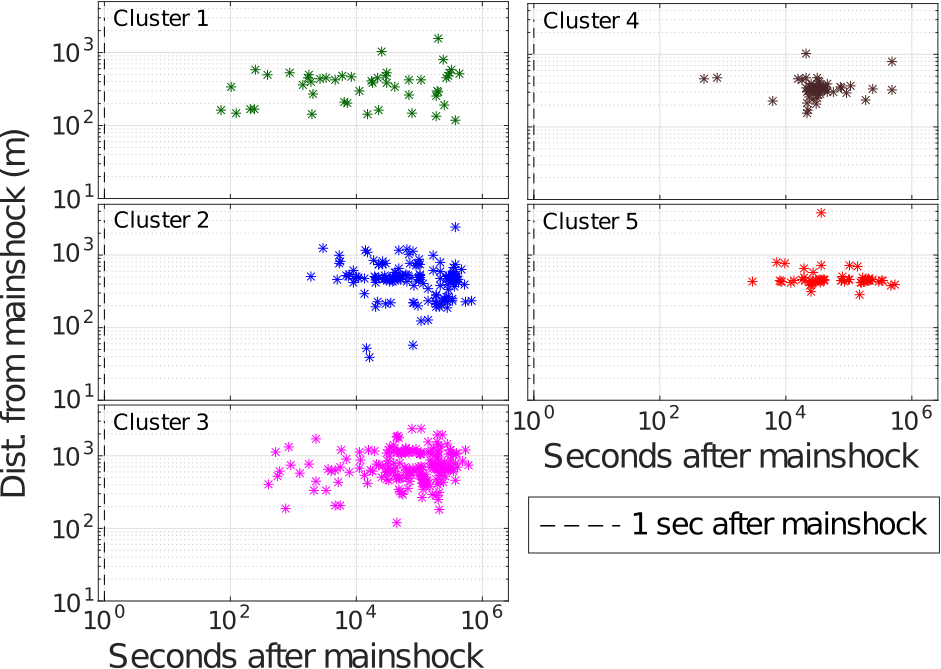
\includegraphics[width=0.7\linewidth]{S3_loglog_time.png} 
\end{center}
\end{figure}
\Assignment{Hugo} \WorkInProgressRevTask
\end{Answer}
%
%




\begin{ReviewerComment}{2}
\noindent 
Be consistent with defining small and medium (or moderate-sized) earthquakes. Line 24 has small earthquakes classified as  Mw<5, Line 54 has medium-events listed as Mw < 6, and Line 83 has small-magnitude events classified as Mw<6. It is most common to consider M 4-6 as moderate-sized and Mw < 3 as small magnitude earthquakes. I recommend grouping small to moderate-sized earthquakes as Mw < 6 consistently.

\end{ReviewerComment}


\begin{Answer}
\Assignment{Hugo} \WorkInProgressRevTask
\end{Answer}
%
%




\begin{ReviewerComment}{2}
\noindent 
Figure 1: The topography in this figure is poor resolution. Is better resolution topography data available? If not, it may be better to remove it because it is distracting and does not add much to the figure. I also recommend adding mapped faults - including the Liri fault. Add scale bar to the main map.

\end{ReviewerComment}


\begin{Answer}
\Assignment{Hugo} \WorkInProgressRevTask
\end{Answer}
%
%



\begin{ReviewerComment}{2}
\noindent 
Figure 3: It is difficult to differentiate aftershock clusters on (3b); expand the time series so temporal patterns are visible. Alternatively, you can plot cumulative events per cluster rather than combining them together.  

\end{ReviewerComment}


\begin{Answer}
We agree with reviewer \#2. We modified figure 3 in the main manuscript so that the cumulative number of events per each cluster can be better seen. In this response letter, Figure \ref{fig:fig3_improved} illustrate the new version. In addition, we include into the supplementary material a figure where a zoom in to the cumulative plot is illustrated for the first 24 hours after the mainshock (figure \ref{fig:fig3_zoom} in this response letter). 
\begin{figure}[!h]
\begin{center}
 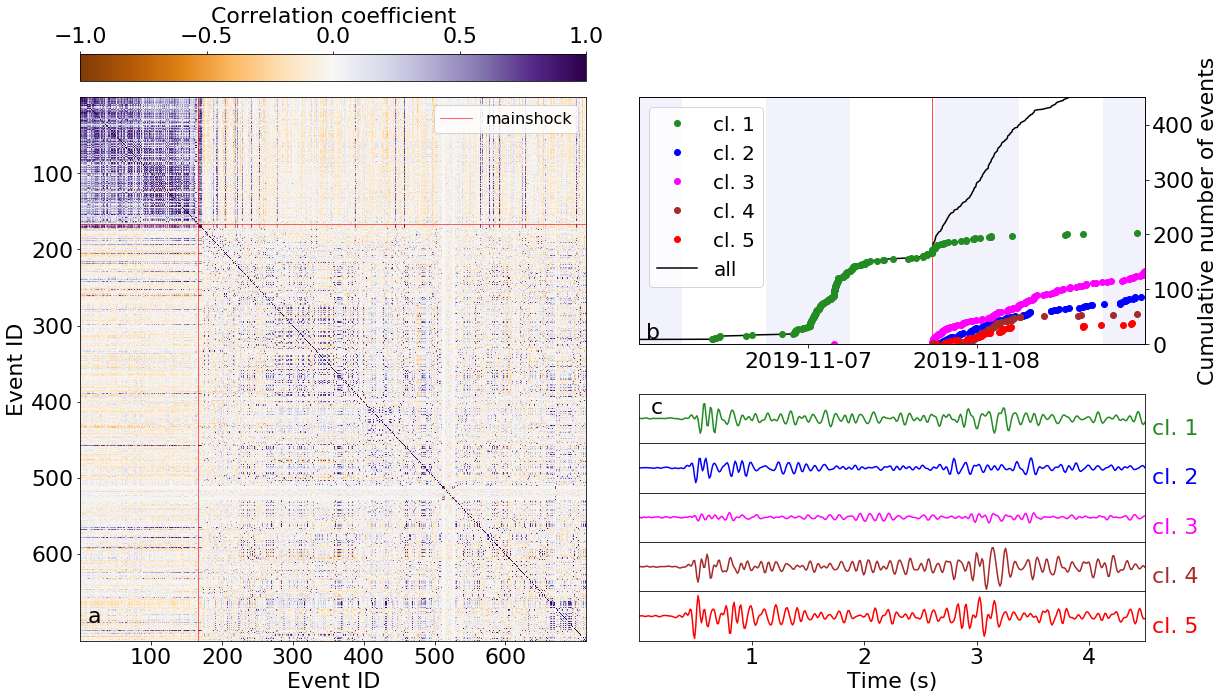
\includegraphics[width=1\linewidth]{wigg_cc_mat_cluster.png} 
\end{center}
\label{fig:fig3_improved}
\end{figure}
\begin{figure}[!h]
\begin{center}
 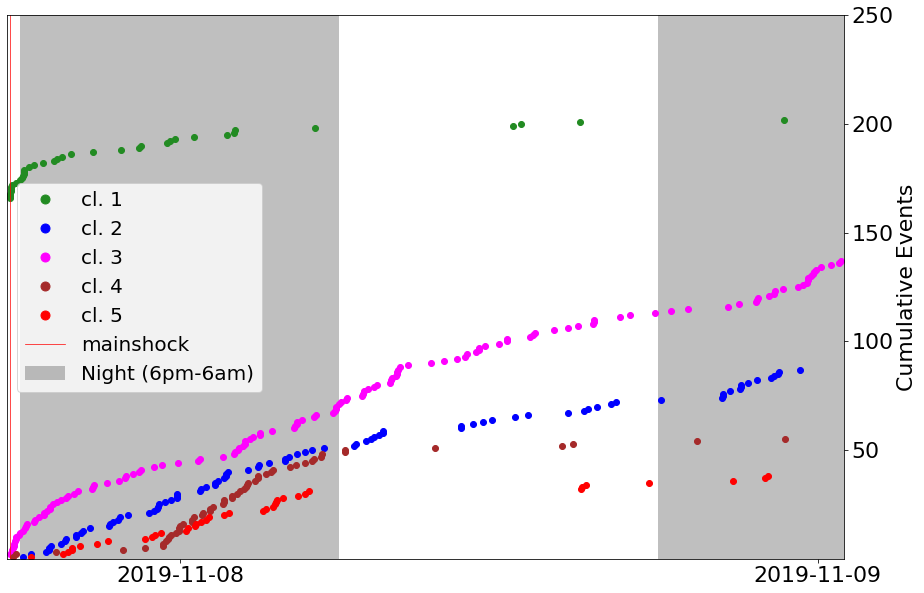
\includegraphics[width=1\linewidth]{S4_cumulative_per_cluster_zoom.png} 
\end{center}
\label{fig:fig3_improved}
\end{figure}
\Assignment{Hugo} \WorkInProgressRevTask
\end{Answer}
%
%



\begin{ReviewerComment}{2}
\noindent 
Supplementary Figure S1: The distance threshold is listed here as 5.3 but is given as 5.5 in the main text (line 166). Please fix this. Change "form dendrogram" to "FROM dendrogram"
\end{ReviewerComment}


\begin{Answer}
Thank you for this comment. We modified the main manuscript according to the correct value used for the clustering and we fixed the typo. We also modified the dendrogram figure to respect the color code used in all the other figures. This figure is part of the supplementary material (figure S1) and it is also included in this response letter as figure \ref{fig:dendrogram}.
\begin{figure}[!h]
\begin{center}
 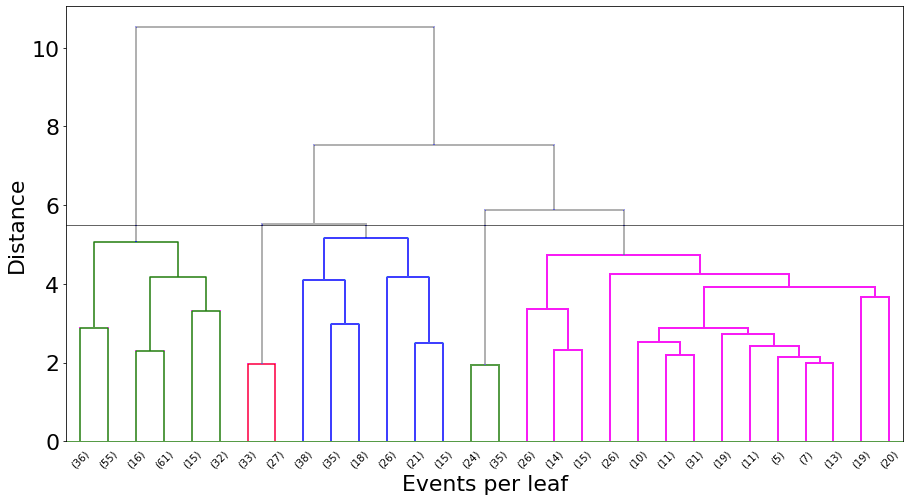
\includegraphics[width=1\linewidth]{dendrogram_balsorano.png} 
\end{center}
\label{fig:fig3_improved}
\end{figure}
\Assignment{Hugo} \WorkInProgressRevTask
\end{Answer}
%
%



\begin{ReviewerComment}{2}
\noindent 
Supplementary Figure S2 is not discussed in the main text. Based on the figure and figure caption alone, the purpose of this figure is not clear. Either add in a reference to it in the main text, or consider removing it.

\end{ReviewerComment}


\begin{Answer}
\Assignment{Hugo} \WorkInProgressRevTask
\end{Answer}
%
%


\subsection*{Minor edits}

\begin{ReviewerComment}{2}
\noindent 
*        Lines 37-38: "…each cluster in this sequence has a distinct triggering mechanism." In the Conclusion clusters 2\&3 and 4\&5 are grouped together in terms of triggering mechanisms; therefore, each cluster does not have a distinct mechanism.  

\end{ReviewerComment}


\begin{Answer}
\Assignment{Hugo} \WorkInProgressRevTask
\end{Answer}
%
%



\subsection*{Specific comments:}

\begin{ReviewerComment}{1}
\noindent Minor edits (suggested additions are in all caps): \\
\begin{item}
\vskip -0.5cm \item \noindent Line 40 - I suggest changing "incoming" to another term that expresses more of an expectation in time, such as upcoming, imminent, impending, or forthcoming. \\ 
\item \noindent Line 41 - "behind the triggering AND NUCLEATION of earthquakes" \\
\item \noindent Lines 40-41: This introductory sentence would be more compelling if you add in the importance of precursory signals beyond models. Yes, models are important, but they are important because characterizing earthquakes is important.\\
\item \noindent Line 47 - What is meant by "more significant?" Most compelling? Most impactful? \\
\item \noindent Line 54 -  change "even for" to "PARTICULARLY for MORE frequent" to emphasize that small to moderate-sized events occur more frequently than larger events and are therefore useful to study. \\
\item \noindent Line 55 - "Improved observations MAY shed light on the physical processes that occur during the triggering AND NUCLEATION of earthquakes…" \\
\item \noindent Line 73 - "ASEISMIC slip processes" \\
\item \noindent Line 85 - Remove "last" before "more recent studies " \\
\item \noindent Line 101 - Change "~15 km" to the actual hypocenter depth of 14 km \\
\item \noindent "Poli et al., 2020b" - Fix citation throughout
\end{item}
\end{ReviewerComment}

\begin{Answer}
\Assignment{Hugo} \WorkInProgressRevTask \\ \vskip 0.5cm
\noindent Thank you for the comments. These suggestions were applied in the revised version of the main manuscript. \\
\end{Answer}
%
%

\bibliography{../bibliography}
\bibliographystyle{apalike}


\end{document}










